\documentclass[UTF8,a4paper,12pt]{ctexbook}
\usepackage{amsmath}
\usepackage{amsfonts}
\usepackage{enumerate}
\usepackage{booktabs}
\usepackage{graphicx}
\usepackage{hyperref}
\usepackage{autobreak}
\usepackage{titlesec}   %设置页眉页脚的宏包
\usepackage{geometry}
\usepackage{fancyhdr}

\newcommand{\keywords}{\large \textbf{关键词}:布偶, 英短, 莫布利}
\newcommand{\ekeywords}{\large \textbf{Keywords}: World Cup, Lancet, Blues}

\renewcommand{\chaptermark}[1]{\markboth{\small 第\,\thechapter\,章\q? #1}{}}

\fancypagestyle{plain}{
	\fancyhf{}\renewcommand*{\headrulewidth}{0.75bp}
	\fancyfoot[C]{\thepage}
		\fancyhead[CE]{北京大学博士研究生开题报告}
		\fancyhead[CO]{\leftmark}
}
\pagestyle{plain}

\title{博士研究生开题报告}
\author{修格致}
\date{\today}

\begin{document}
\thispagestyle{plain}
\makeatletter
    \begin{titlepage}
        \begin{center}
            
\includegraphics[width=0.6\linewidth]{Figs/Logo.png}\\[4ex]
            {\Huge \bfseries \hspace{3ex} \@title }\\[10ex]
        {\huge \centering
        \begin{tabular}{cc}
                \makebox[5em]{\textbf{题目:}}        & \underline{\makebox[10em]{\textbf{介观尺度的城市交互问题}}}
        \end{tabular}
        } \\[20ex]
        {\Large \begin{center}
            \begin{tabular}{cc}
                \makebox[5em][s]{\textbf{姓名:}}        & \underline{\makebox[10em]{\emph{修格致}}}\\[1ex]
                \makebox[5em][s]{\textbf{学号:}}& \underline{\makebox[10em]{1801110566}}\\[1ex]
                \makebox[5em][s]{\textbf{院系:}}      &\underline{\makebox[10em]{\emph{地球与空间科学学院}}} \\[1ex]
                \makebox[5em][s]{\textbf{专业:}}      &\underline{\makebox[10em]{\emph{地图学与地理信息系统}}}\hfill \\[1ex]
                \makebox[5em][s]{\textbf{研究方向:}}      &\underline{\makebox[10em]{\emph{数字地球与智慧城市}}} \\[1ex]
                \makebox[5em][s]{\textbf{指导教师:}}
                &\underline{\makebox[10em]{\emph{刘瑜\quad 教授}}}
            \end{tabular}
            \vfill
        \end{center}
        }
        {\Large\today}
    \end{center}
    \end{titlepage}
\makeatother
\thispagestyle{empty}
\newpage

%Add content for page two here (useful for two-sided printing)
\thispagestyle{empty}
\newpage
% \chapter*{摘要}
\setcounter{page}{1}
\pagenumbering{Roman}


% {\vfill \keywords}

% \chapter*{Abstract}

% {\vfill \ekeywords}
\tableofcontents

\chapter{选题背景}
\setcounter{page}{1}
\pagenumbering{arabic}


% \section{选题背景} % 要写三页

% 什么是介观,介观视角下城市的现象

介观尺度的概念由Van Kampen于1981年所创,指的是介乎于微观和宏观之间的尺度。针对城市科学,介观尺度是指城市内部几公里范围内的空间尺度,这是城市研究和城市规划中最常用的空间尺度。微观的个体在小空间尺度交互,形成介观尺度的混合用地功能、回转半径;介观空间结构作为城市整体的功能分化单元,通过其间的交互,完成城市整体的功能。处于介观尺度的地学现象,尽管包含很多更小的研究单元,但其系统尺度小于相干尺度,介观尺度单元的同一样本中的空间单元保持较强的相关性,但各个空间单元的差异极大,城市系统的全局平均性质不再有效的刻画系统中所有微观空间单元的性质。理论角度看,在介观尺度下,城市的人口和社会经济密度保持了足够的异质性(如用地功能分化等);而对于该尺度的城市现象来讲,个体行为特征的聚合又可以体现出足够的规律性。实际角度看,介观尺度对于政策制定、感知城市空间、场所性等非具体、弱化实际度量的方面又有着很好的反馈效果。这使得基于街区、人口普查单元等介观尺度空间单元及其之间交互的研究体现出重要的意义。

在快速城市化过程中,全世界的大城市和城市群集中涌现出很多有共性的模式与问题。其中包括空气污染、城市热岛现象、能源消耗问题、社会空间不平等以及很多与可持续发展有关的问题。为了向决策者提供可靠的理论和新范式来缓解这些城市问题,对城市结构与演变规律进行建模成为尤为重要的一环。基于简单规则而可解析的统计物理模型可以在不同的角度给出城市发展机制的阐释和预判。近年来,可供城市研究参考的数据越来越多,建模的置信程度也在逐渐提高,这使得此类简洁有力的物理模型能够提供更好的连接理论和经验结果的工具和概念,从而在城市研究发挥重要作用。因此,构建可定量研究、能解释尽量多的城市现象、并有预测性的城市科学是城市研究中极具潜力的发展方向。城市是由环境和其中的人组成的。个体行为的总和构成了城市的动态。基于个体行为模式的挖掘,科学家在人类移动模式、职住平衡分析等方面建树颇多。然而,从数据来讲,由于个体数据采集成本较高、隐私保护等问题,基于个体的研究受数据制约比较大;从研究效果来讲,基于个体行为模式的研究结论整体可复现性不高,研究结论受随机误差影响比较大,同时空间一致性不强,很难得到较为通用的、有意义的模式。在此背景下,选取合适的研究尺度,从城市的内蕴框架下探究城市模式的涌现,就成了一个更好的选择。

% 广泛的适用性,普遍存在的问题

已有研究从介观尺度结构出发,已经挖掘出来很多有意义的模式。可以概括为如下三类:\begin{enumerate}
    \item 从空间分布(一阶量)来看,介观尺度模型可以反映空间上连续变化的事物的分布。在刻画空气污染\cite{mijling2012using}、城市热岛效应、城市形态演化\cite{raimbault2018calibration}、人口模式识别方面都是建模的核心。
    \item 从空间交互(二阶量)来看,介观尺度对应着聚合尺度的空间交互,在流行病传播、对政策制定等角度有着核心意义。% 传统数据比较匮乏
    \item 从介观尺度模式的形成来看,介观尺度观测很好地体现了城市微观-宏观之间的跨尺度特征,在城市分区功能分化、交通拥堵、交互尺度提取等方面方兴未艾。
\end{enumerate} 这些模式的提出隐含了介观尺度观测城市问题的普适性:既是个体交互的总和,又是构成城市整体性质的元素。

% 存在很多广泛的其他领域的方法可以处理其中的问题,但存在一些问题,使得已有的方法做出来的结果不能有普适性的意义。

社会物理(social physics)与地理大数据(big geodata)的结合有助于我们建立统一的框架来理解介观尺度规律。然而,这个框架中已有的方法和工具暂时不足以完全解决城市科学家的观测需要。其中几个主要方面为:\begin{enumerate}
    \item 数据空间与真实空间的非线性对应关系。
    \item 介观尺度结构空间交互的高耦合性。
    \item 统计涨落对城市介观尺度结构稳定性的影响。
\end{enumerate} 首先,随着移动互联网时代的到来,地理学者可以在社会感知的框架下处理的数据不计其数。如果将这些数据汇总到一起,则凸显出数据中的结构,及其在真实空间中的对应,是很困难的。以英国的人口普查数据为例:每十年,政府会对每个目标区域统计约1450个变量。如何在研究特定问题时确定足够好的变量,以及他们的权重,是一个亟需解决的问题;其次,移动大数据观测了多尺度人类行为,但其中规律性的部分的提取、以及对随机性的预测仍然是衡量城市软性质的主要桎梏\cite{song2010limits,barter2019manifold,dalziel2013human}。最后,在拥有对城市生活和人类社会如此多的观测数据的前提下,很多城市模式的生成模型需要更多数据的检验\cite{makse1995modelling,wilson2003development,rozenfeld2008laws}。

% 软与硬的对应:数据中硬的东西挖掘不出来了,需要理论高度和非线性映射来寻找城市内蕴的合适的结构。

总之,在大数据的帮助下,我们有了很高的潜力来更好地建模城市。但同时,提出更精确更合理的模型,以及检验以往猜测的准确性是进一步研究的重中之重。理解城市介观交互模式中涌现的软性质,并对其机理性提出解释,则是将城市研究科学化的核心观念。


% 因此,我们需要开发新的方法,
\chapter{研究现状与问题归纳}

\section{研究现状:城市介观尺度的空间交互问题}

根据联合国的最新报告,2018年全球人口为76亿,城市人口为42亿,而城市人口所占比例还有不断上升之势\cite{unreport2018}。城市可持续发展与人类的未来息息相关。然而,由于社会经济发展水平和区域背景的不同,不同城市发展的进程是不平衡的\cite{seto2013book}。对于许多城市来说,区域经济发展不足以满足日益增长的城市人口的需要,以至于出现基础设施建设不足、环境污染、社会分化等问题\cite{zhao2021global}。通常来讲,基础设施建设的速度相对于人口增长的速度是亚线性的,而个体与地理区域之间的交互带来的经济、创新等因素的增长则是超线性的\cite{yakubo2014superlinear}。基础设施的固定空间属性和空间交互的常返性使得城市发展的不平衡体现出空间聚集的特征\cite{gonzalez2008understanding, wang2016process}。在本文中,我们用\textit{介观尺度}一词来指代类似社会经济属性空间范围的特征尺度,相对于城市中的人、车、建筑等微观个体,以及宏观上的城市整体而言,介观尺度介于宏观和微观之间,可以是城市内部的街区、社区、街道、交通小区、生活圈、商圈、单位大院等各种功能单元,也可以是均匀划分的地表网格,一般在百米到十几公里之间。\cite{raimbault2020empowering}。城市发展过程中,空间交互和社会网络在使城市充满活力的同时也加剧了由于城市人口规模增长过快而出现的犯罪,拥挤,低空气质量和较高的生活费用等诸多问题\cite{toth2021inequality}。如何摒除过多的随机性,从系统上理解空间交互,对于研究城市中的知识涌现、信息和疾病的传播、贫民窟等空间分化等现象有着至关重要的作用。

城市中的空间交互问题在不同的聚合尺度上通常有着不同的研究结论。以人类移动性研究为例:个体层次的移动性常用列维飞行来近似\cite{brockmann2006scaling,gonzalez2008understanding,mantegna1994stochastic,metzler2007some},其中体现了高度的随机性;而在群体层次,人类移动性则在出行目的、社群性质、频率分布等方面体现了较高的规律性\cite{peng2012collective, jiang2017collective, dong2020spectral, wachowicz2016finding}。这些群体的移动性汇集成了介观尺度空间单元的空间交互。介观尺度是交互的视角下一个承上启下的尺度:小于介观尺度(数公里范围内)个体出行的目的地有着比较强的随机性和各向同性\cite{berry1958recent, degroot1974reaching, jurdak2015understanding},而大于介观尺度的出行则可以用种种标度律来解释\cite{gonzalez2008understanding, brockmann2006scaling}。这种性质使得介观尺度在很多核心问题上有着独特作用:例如处理城市流行病传播的状态分类问题时,可以避免基于个体模拟的维度灾难,同时得到有预测性全局的结论\cite{colizza2007invasion, colizza2007reaction, watts2005multiscale}。这与生态学中,基于种群尺度分析群落的稳定性的思路是不谋而合的\cite{may1972will, allesina2012stability}。

随着交通、手机信令、社交媒体、细粒度普查等元数据采集精度的提高,从随机性的个体行为中提取群体行为进行介观尺度的研究也有了足够的可行性。然而,数据在描述不同地理位置的特征时,效力往往是不同的:例如相同空间交互量的两对起讫点可能会因为个体访问频次的差异而对应着不同的出行目的\cite{dong2020spectral};经济指标类似的两个区域也可能由于不同的常访人群而在未来发展方面性质迥异\cite{mantymaa2018integrating}。为进一步深化对空间属性的理解,我们将描述城市某些空间特征的属性划分为硬属性和软属性两种类型,并定义:可以直接由采集数据简单变换得出的城市属性为城市的\textbf{硬属性};反之,需引入空间结构、额外专家信息才能从数据出解读出的城市属性为城市的\textbf{软属性}。前者例如例如基础设施、交通规划和分区;后者则更常与居民的社会交往,例如社会凝聚力、城市精神和氛围等相关\cite{barter2019manifold}。城市的软属性对于城市的居民幸福感、应对灾害能力、可持续发展、城市吸引力等方面都发挥着重要作用。因此,在发展基础设施建设的同时,考虑从优化空间结构,提升对城市交互确定性和随机性的理解等方面实现城市软属性的提升是一个有价值的目标。然而城市软属性的提取并非易事\cite{kim2014perceived,begg1999cities,fujita1999spatial}。

在属性提取和数据聚合的基础上构建研究介观尺度的空间交互问题,应至少包含以下三个议题:
\begin{enumerate}
    \item 通过现存的社会经济特征划分介观尺度空间单元。将普查、社会感知等采集尺度更小的空间单元聚合成介观尺度空间单元,以得到相对一致的社会经济描述;
    \item 将介观尺度空间单元之间的交互关系用复杂网络进行建模,并分析该网络上的传播过程、稳定性等性质;
    \item 探究局部一致性比较强的介观尺度空间单元的形成原因与机制。
\end{enumerate}

%--------------------------------------------------------------------------------------------
\subsection{从多元地理大数据中提取城市介观结构}

个体的交互在过小的尺度上常有较强的随机性,通常用扩散过程来描述\cite{helbing1995social};但是从空间角度,这种个体的随机行为却助推了城市用地功能分化的进度,使得各个区域有了相对稳定的发展趋势和方向,分担了特定的城市功能\cite{louf2013modeling}。如前文所述,这个过程也可以解读为城市的软属性逐渐变成城市硬属性的过程。通过数学模型,很多学者阐释了城市的软属性如何有序组织排列城市的硬属性,这些不同城市元素的空间组织可以帮助决策者理解城市的韧性和健壮程度\cite{batty1971modelling, louf2013modeling}。经济学家使用大量的多变量模型来预测扰动对城市系统的影响,比如土地利用与交通的相互作用、产业结构调整对城市单-多中心模式转换的影响等\cite{fujita1982multiple, acheampong2015land}。这些预测可能非常准确,但依赖于对大量参数的拟合。而城市经济学家和经济物理学家更倾向于使用简单的规则和变量,基于城市居民的个体选择的群体效应来复现城市现象。这些模型体现了比较强的解释能力,但缺点是无法完全重现城市的多样性,以及难以证伪。因此简单规则导出的模型预测通常不适用于为具体的干预措施或政策提供建议。

另一个思路是从物理学借鉴思路,挑选若干变量建立动态模型,然后根据对少数变量的分析制定定性或定量预测\cite{riccardo2012towards, castellano2009statistical, jay2020neighbourhood}。这种方法的优点在于结果不是从黑箱中产生的,而是通过理解过程的动态而获得的。对软城市特性的出现进行建模的一个核心挑战是识别一组能够捕捉这些特性的变量。通过将城市的文化和经济方面进行量化建模面临着无数的可能性:可以选取很多变量,如家庭收入、家庭规模、就业状况等,这些变量之间都有很强的相互依赖性。另外,不同因素对于不同区域的支配可能是空间异质的:比如城市核心区域的发展潜力可能更依赖于绿地覆盖面积,而郊区发展潜力则更依赖于其他基础设施的密度。因此,该类方法的挑战在于找到决定城市特定区域整体性质的关键人群。

近年来,随着机器学习技术的普及与发展,以及社会感知等认知框架的建立,地学人工智能在地理学领域提供了广泛的应用场景。“城市数据挖掘”描述了一种揭示一组地理空间数据内部的模式和规律的逻辑或数学和部分复杂的描述的方法论\cite{behnisch2009urban, bendimerad2016unsupervised}。基本的线性回归之外,诸如涌现自组织映射(Emergent Self Organizing Maps)\cite{ultsch2005esom}、局部线性嵌入(Local Linear Embedding)\cite{roweis2000nonlinear}等方法的引入逐渐使人意识到,在城市数据的参考系下,城市并不存在一个全局适定的度量。多维时空数据不均等地反映在不同区位的优势与劣势。进而使得以下成了很重要的问题:如何针对不同的空间区域选择合适的统计指标来反映城市某个侧面的性质?

第一个尝试是手动选择关键指标。\cite{bosetti2020heterogeneity}中对流行因素和人口统计学指标进行了回归分析,证明了免疫力、人口分布、和人口流动的异质性的影响下,麻疹爆发的概率会显著被低估。但是,此类方法容易失去更深层次的因果关系。因此,我们需要一个客观的方式选择关键变量。这样,添加到模型中的每个变量都会最大限度地增加我们描述城市差异的能力。第二种尝试是利用机器学习方法进行降维。其中代表性的方法为主成分分析(Principal component analysis, PCA)。\cite{deng2008pca}利用多元卫星数据,结合了PCA方法进行了用地功能分类研究;\cite{nagendra2003principal}用PCA方法分析了高耦合性的交通、排放和气象数据,结果显示,24小时平均的四个主成分对交通和排放变量的载荷最高,且它们之间有很强的相关性;\cite{palmason2005classification}分析了城市形态特征,得到了比较好的抽象表述。此类方法的优点是可以简单而直观地找到关键的数据法向量。但其有一个不容忽视的缺点:该类方法的实现本质是为统计数据建立一个全局普遍适用的度量,以寻求找到最佳权重关系,因此其无法很好地反馈城市中大多数非全局、非线性的地理耦合关系。

近期,以扩散映射(diffusion map)\cite{barter2019manifold}为代表的流形学习方法在非线性地理大数据融合方面给出了一些答案。在多元、多源地理大数据的融合过程中,不同的数据来源会反映城市现象的一个方面,进而特征空间上的城市形态可能是非欧几何:某些数据集或统计指标非常突出地显示城市的某个小区域的优点,而在其观测下大量的其他区域则非常均质。这使得定义一个局部度量显得尤为重要。在已有工作\cite{barter2019manifold}中,通过考察英国人口普查数据的1450个统计量的结果,作者通过扩散映射方法找到了最重要的两个城市特征对应的人群:大学生及大学雇员、以及保障性住房住户。该方法有很好的物理直观,也能找到数据中的非全局特征。本质上,该方法捕捉了个体交互在小尺度上的的各向同性及其诱导的局部相似性,从而将微观空间单元聚合成了介观尺度空间单元。根据我们与原作者的一些讨论\footnote{邮件及网络会议等形式},扩展该方法可以容易地得到更多城市特征,亦可以定量地解释人文地理中难以量化描述的城市现象,比如空间对偶\cite{lomi2000density}、城市多中心性等\cite{gordon1986distribution, mcmillen1997nonparametric}。该方法可以摒弃人为因素选择通常具有空间连续性的城市空间,是研究一大类介观尺度交互空间问题合理的空间依据。

\subsection{空间交互视角下城市系统韧性与稳定性}

“城市韧性(Urban resilience)是指城市系统及其所有组成部分在时间和空间尺度上的社会生态和社会技术网络在面对外界干扰时保持或迅速恢复到预期功能的能力,适应变化的能力,以及迅速转变限制当前或未来适应能力的系统的能力”\cite{meerow2016defining}。城市地区除了作为资源消耗节点和创新场所之外,在理论和实践上都已成为人类系统韧性的实验室\cite{meerow2016defining}。一些城市系统的研究显示,城市现有交互模式被证明与贫民窟的形成有着很高的关系\cite{brelsford2018toward}。亦有研究表明,长期发展下,旧城市将不可挽回地被新城市取代\cite{fujita1997structural, cottineau2017diverse}。这些现状使得探讨未来城市设计时,有必要加入对“韧性”的讨论。韧性在城市科学中具有积极的社会内涵,代表着城市面临流行病、产业升级、区位重心转移等问题时,回到正轨的能力\cite{mcevoy2013resilience, o2013deconstructing}。高速增长的城市规模使得城市核心结构的人口和经济规模的密度到达了一个非常高的水平。理论角度而言,规模更大的系统往往是开放而非均衡的\cite{louf2013modeling,may1972will}。如何在这种非均衡的系统中找到\textbf{结构稳定性}就成为了城市保持韧性最重要的议题。

现有研究中,城市是否可以保持韧性可以通过衡量城市对抗外界冲击的能力来衡量。冲击对城市的影响可以考察其对应的传播过程\cite
{massaro2018resilience}。以流行病传播为代表的传播过程在城市交互系统中往往体现出复杂的性质。控制流行病传播的政策则往往建立在介观尺度的空间范围,如小区、交通小区、街道、人口普查单元等。流行病传播的过程,是通过人与人交互以及人在各种尺度上的移动从而产生的空间交互实现的\cite{belik2011natural}。另一方面,疾病的控制也可以理解为缩减疾患出现的区域,使之不影响人们的正常生产生活。在历史上,我们也有一些成功的先例,如斯诺利用地理信息系统的思路将1832年伦敦霍乱的源头定位到贫民区布劳德大街上的公共水井。而如今,贫民地区依然是疫情爆发的重灾区\cite{sahasranaman2021spread}。城市生态学者的一些研究中发现,除了卫生条件差之外,贫民地区在城市拓扑上也有着独特性质,通常是城市中流动性最差的区域\cite{brelsford2018toward},是城市交互系统的“势阱”。这种区域中交互的保守性更加催生了流行病和犯罪的集中爆发。但我们对疾病爆发的非线性性、周期性、相位问题等方面的理解依然比较匮乏\cite{dalziel2013human}。一个世纪以来,流行病、犯罪等传播过程的模式发生了很大的变化。以麻疹为例,模式转化主要存在于规则的周期和不规则的、混沌的周期之间,以及从小区域同步振荡到复杂空间上的不连贯爆发。如果将麻疹传播等过程看做不同舱室人口组合的一种自然生态系统,则其在不同的时间地点表现会表现出迥异的发展态势。但一些基于简单空间交互和正弦周期性感染力假设的模型就可以完美预测这些动态过程的非线性分岔。B. Grenfell模型\cite{earn2000a}可以将这种转变解释为出生和疫苗接种率变化的后果。而如今,随着城市化进程的更进一步推进,便捷的城市交通也加剧了流行病的蔓延的速度,也增大了控制的难度。城市内部组分之间的流量构成是异常复杂的,随着不同的观测尺度有着非常大的异质性\cite{masucci2013gravity}。网络科学的视角来看,诸多人类的交互网络(由于人们对效率的追求)都是无标度的。而根据网络上流行病学的基本结论:无标度网络上的流行病传播是不存在阈值的,即疾病最终会传染被网络连接的所有人\cite{eguiluz2002epidemic, plucinski2013clusters}。流行病作为城市突发问题的典型代表,可以提示我们在城市区位设计的时候,不能完全遵循自组织的连接方式。其也应该有动态变化能力,以适应突发状况的出现。

涉及政策实施的流行病模型大都需要舱室化为元人口(meta-population)模型:每个元人口代表一个空间范围的人的集合,利用网络对其交互进行建模,并提出控制方案,以使得基本复制率$R_0$小于$1$. 如前一节所示,有意义的空间范围也往往是介观尺度的空间单元。其交互有着自然的生态学对应:物种之间的捕食、互利共生等关系亦有着用网络描述的历史\cite{may1972will, allesina2012stability, coyte2015ecology}。利用动力系统中不动点的稳定性理论,理论生态学中给出生态系统中各个物种的种群密度保持稳定的充分条件。一个合理的设想是:城市中各个区域的流行病患病人数作为交互的种群,并利用空间交互推导出其交互作用,探究流行病群落在零点是否可以保持稳定。如果可以保持稳定,则该城市对于流行病具有韧性;反正如果无法保持稳定,则城市对该流行病不具备韧性。该方法直观而清晰地阐释了城市流行病传播爆发的动力学本质。因此我们也有必要回顾一下相关的生态学理论。

系统稳定性的讨论始于\cite{may1972will}。该文章基于 Gardner 和 Ashby 实现的计算机模拟动力系统的结论:大型复杂系统只能在一定临界程度的连通性上面是稳定的。而城市系统的高联通度使其在面对外在冲击时有着天然的桎梏。虽然基于交互矩阵的生态系统结构分析已经有了比较悠久的研究历史,空间因素在生态中的真正意义还少有人解释。\cite{lin2019spatial}给了一个空间版本的社会困境的解答。其中隐含了两层深刻的意义:生态的时间性,系统在演化的过程中存在着周期性。这意味着区域发展过程存在着势能积累。另一方面,空间性给系统提供了缓冲空间,使得博弈的不利方的损失可以以类似“势能”的方式积累。这与系统的韧性\cite{gao2016universal}概念是不谋而合的。这个文章的结论可以解读为:自然系统的韧性来源于系统的空间性。\cite{feng2020comprehensive}提出了一个 "尺度-密度-形态 "的城市韧性框架以及指标模型,基于景观生态学和演化韧性的理论来研究城市韧性的演变。该工作提出的控制城市无序扩张、降低人口和建筑密度等提升城市韧性的措施与\cite{may1972will}中的稳定性准则也是相符的:物种越多、连通性越高、交互强度越高的随机生态系统越难稳定。\cite{allesina2012stability}中主要对物种间交互的相关关系进行了讨论:物种对相关关系越为负相关,对应生态系统越容易达成稳定状态。对应到城市科学中的结论应为交互流的对称性越差,城市系统越容易达到稳定状态。

演化生态学近期的一些发展连接了微观尺度个体的空间交互和系统的整体性质,并解释了诸如“公地悲剧”等传统社会学问题。城市间动态平衡是我们理想的状态。但是城市发展过程中出现的很多问题也是我们不能忽视的。经济周期的出现、城市收缩、城市发展不均衡等现象的出现使我们反思,城市发展中是否有着难以避免的固有问题。公共地悲剧(tragedy of the commons,TOC)是Hardin\cite{hardin1968tragedy}探索并定义的一种社会困境,它发生在两个人或群体选择不同的策略来利用有限公共资源的时候。个人出于自身利益耗尽公共资源,综合收益将劣于个体间合作、有节制地利用资源得到的利益。这种问题的根源在于人类价值观的贪念使得增加公共资源的时候,增加的生产意愿不一定会提高。所谓“三个和尚没水喝”。城市发展也有着一些对应的场景。比如说城中村、贫民窟等现象,就是城市无法使得所有人都努力工作,却提供了过得下去的生活条件,使得贫民仍愿意居住在城市之中而导致的。有一些新的研究确定了一些条件。在这些条件下,城市虽然仍不会百分百随着自身的发展而一帆风顺、长治久安,但却能走出困境\cite{lin2019spatial}。为达成这些条件,我们需要考虑个体交互作用下局部群体模式的形成规律。

\subsection{个体交互作用下介观尺度模式的涌现}

城市内介观尺度空间单元会在很多方面形成固定的空间模式,比如方言分布\cite{burridge2017spatial}、政治意见\cite{rogers2013consensus}、贫富分布\cite{kirkley2020information}等。这些空间聚集模式通常被认为与城市空间的自组织特性相关:即城市作为一个混沌系统,会自发形成平衡的耗散结构。在社会理论中,尼古拉斯·卢曼引入了“自我指涉” Self-referentiality的概念作为自组织理论的社会学应用\cite{luhmann1984soziale}。对于卢曼而言,社会系统的“交流”是自我复制的,即交流产生进一步的交流。因此,只要存在进化的交流,社会系统就可以自我复制。对于卢曼而言,人类就是系统环境中的传感器。这与我们熟知的社会感知框架也不谋而合。卢曼通过功能分析和系统理论发展出一套关于社会及其子系统的进化论。自组织现象意味着特定特征尺度的现象涌现。我们摘取一些具有空间背景的例子:\cite{friesen2018similar, pelz2019similar}验证了全球主要大城市的贫民窟规模都是类似的,并会形成图灵不稳定性的图案;\cite{louf2013modeling, courtat2011mathematics}等工作通过交通与机会模式的平衡解释了城市多中心现象的出现;\cite{rosvall2005networks}根据人在路网中导航所需要的信息量证明,城市网络并不是为了沟通而优化的,而局部地理环境比网络拓扑有着更重要的意义。这些结论告诉我们,寻找驱动介观地理模式形成的原因有助于我们对城市组分交互的“属性”信息得到更好的先验知识。

“回音室效应”\cite{wang2020public, liu2020modeling}作为信息传播领域的一个研究热点,其中的研究方法和对人群的理解亦可以应用到理解介观模式形成问题中。由于人的从众心理和地理相关性的存在,地理空间单元容易产生极化和同质的意见集群,通常被称为回音室。回音室效应可能阻止人接触与其现有信仰相反的信息或观点,并进一步激化具有极端信仰的个人。在高度信息化的社会中,回音室效应在各种时空尺度加速出现\cite{wang2020public}。已有研究中,社会影响模型\cite{noah2006structural, friedkin2011social, parsegov2016novel},阿克塞尔罗德的文化传播模型\cite{axelrod1997dissemination},有界信心模型\cite{deffuant2000mixing}等理论工作确立了解释微观尺度偏差积累到宏观尺度的基础。在这些人类移动的行为模式涌现的过程中,如何防止城市动态固化、局部同质化将是规划者保持城市活力的重要考虑方面。

为此,经济地理学家基于同质化人口给出了一些模型来定量解释城市模式固化的条件。以谢林模型(Schelling model)为例\cite{schelling1971dynamic}:该模型假设每个个体都温和地倾向于与自己同种族的人做邻居,但作者通过大量数值模拟发现,无论这个偏好有多么温和,每个小区中都会出现被单一种族占领的情况。该结论在大量的自然生态系统中找到了对应\cite{traulsen2006stochastic,baxter2008fixation,lombardo2015fixation},因此我们也期待保护生态学中的调节思想可以更多地应用到城市人口生态性建设上。

\section{问题归纳}



介观尺度聚合地理大数据和理论模型方法可以挖掘个体行为模式的确定性、城市的空间结构、以及城市作为一个系统的性质,有助于理解城市面对外来冲击、政策变化等因素的反应。不过,自适应空间单元的提取、城市交互系统稳定性指标、交互模式中的涌现现象等问题还欠缺足够好的处理方法。

\subsection{介观空间单元的提取}

虽然现有丰富的数据源提供了很大的便利,但是这些数据本身的复杂性也是一个挑战。为了深入地通过大数据了解城市的社会结构,至少需要克服以下两个问题:1. 特征效力的空间异质性。高维特征空间的大部分特征只在少数空间区域有反映空间差异的能力,而在更多的空间区域效果平庸。如果手动选取主要特征则会产生如下问题:2. 解释变量的主观性:选择明显与空间区域的差异性相关的特征可能会导致相反的结论。如何找到其中的主要变量,并摒弃选择的偏见,得到一个相对客观的结果,是一个不易解决的问题。

扩散映射法已经提供了一个很好的基础,并在英国、美国的数据集上,针对找到城市结构的关键指标\cite{barter2019manifold}和构建贫困指标\cite{ghafourian2020mathematical}等角度得到了很好的应用。但其针对特定城市问题的理解依然很有限,比如刻画负相似性、不同城市系统的差异性等。例如:作为目的地,不同工作地点的访问人群相关性可能为负,而休闲娱乐场所则拥有正相关性。总之,我们还没有一个足够完善的体系来针对特定任务,利用多元地理大数据找到合适的空间范围。

\subsection{城市介观空间单元交互的稳定性}

定量评价城市的各种政策的效果一直是维护城市交互系统稳定的一个难题。而生态学中的理论显示\cite{may1972will},交互强度过高的系统维持稳定的概率很低。另一方面,从介观尺度进行防控疫情、犯罪等问题又是最为合适的:成本可控,而且管理力度足够。在城市面对流行病等外来可传播冲击时,如何在介观尺度制定强有力、而又不矫枉过正的政策来维护其稳定就成为了一个关键问题。

\subsection{城市介观结构的模式形成问题}

微观交互如何在介观尺度上形成固定的混合模式?目前的大多数研究依靠自上而下的方法:通过大数据挖掘城市用地功能混合模式,而缺乏一个机理性对于多产业、多种意见人群如何共存和如何演化的理解框架,使得这类方法很难具有普适性。也有一些关键问题有待解决:比如如何解释小区域称为特定政党的票仓,而其邻居支持另一个政党。城市复杂机理的理解又是研究政策渗透、资本投放等问题的重要基础。因此我们需要一些随机过程模型来对城市介观单元的混合模式的形成规律进行探究。

% \section{研究方法和技术路线}
\chapter{研究内容}

\section{框架}
% 一页
针对城市中的各种交互问题,找到合适的研究尺度是给出解答的重点。在两个极端的尺度(即个体-微观,与整个城市的特征-宏观)之间,所有的尺度问题都可以用介观尺度的方法论加以解决。

第一个问题是针对问题的空间区域的提取。我们在利用地理大数据进行研究时,采样精度往往与需要探究的问题不完全一致,需要我们聚合成针对问题的合适尺度。比如,对于社会不平等的剥夺指数问题,研究数据主要是普查数据(普查范围是~8000人的无重合空间范围),而与之对应的政策调整范围则是更大的(区、县等数万人到数十万人的)区域。我们利用\textbf{扩散映射}技术,在多元数据中找到合适的参量,以针对需要的问题得到合适的空间范围。该方法不会从多元空间数据中选择特定的\textbf{列},而是从完整的数据集中构造一个针对问题的指标。由于其结构,扩散映射所提取的索引不会引入源数据偏见之外的偏见,并且对于数据操纵的企图具有很高的弹性。

第二个问题是介观尺度下的信息传播与共识达成问题。随着城市规模的增大,城市中各个区域的沟通也变得更加紧密。根据\cite{stark2008decelerating}, 更频繁的微观尺度交互会使得政策贯彻和城市面对外来冲击的弹性降低。为此,我们借鉴Hubbell模型\cite{hubbell2001unified},考虑不同社区中有若干个体,而每个个体针对一件时事(比如,疫情期间政府对于戴口罩的倡议)都有一个\textit{意见},在随机初始状态下意见统一的期望时间。我们发现,加入社区/集合种群等介观结构更容易达成意见统一。其他细致结构也对于我们理解介观结构对于形成城市意见共同体的影响。

第三个问题是介观尺度城市稳定性。城市各组分沟通得紧密也伴随着城市面临外在冲击时,冲击在城市内部快速的传导。城市面对流行病、战争等外来冲击时的抵抗能力通常被概括为城市韧性/稳定性。城市稳定性也对可持续发展的诸多方面(多样性,连通性,去中心化和自给自足)有解释作用。我们试图基于矩阵理论,利用城市中小区块的交互强度提出一种稳定性度量。在此理论下,可以通过求解矩阵的实部为负的特征值所占全部特征值的比例来衡量外来冲击在城市内部爆发的倾向性。

根据我们的理论和实证结果,介观空间单元的交互视角下,城市的空间连续性、一致性、稳定性等特征的结果都与微观尺度交互的结果不同。这说明城市中介观尺度观测结构不容忽视,是城市建模的重要一环。


\section{研究内容}
% 六七页

\subsection{利用扩散映射提取城市隐藏特征}

从认知、规划等角度来讲,城市空间都不是一个典型的欧氏空间:同样的欧氏距离下,穿不穿越河流、人流密集还是稀疏,都会产生不同的时间消耗和其他感知差异。这个事实说明城市空间的刻画是复杂的,全局的空间度量很难刻画城市空间的本质。为了更好的描述城市空间,我们需要更复杂的城市认知框架。数学上基于局部距离定义的\textit{流形}提供了一个可能的方案。

\begin{figure}
    \centering
    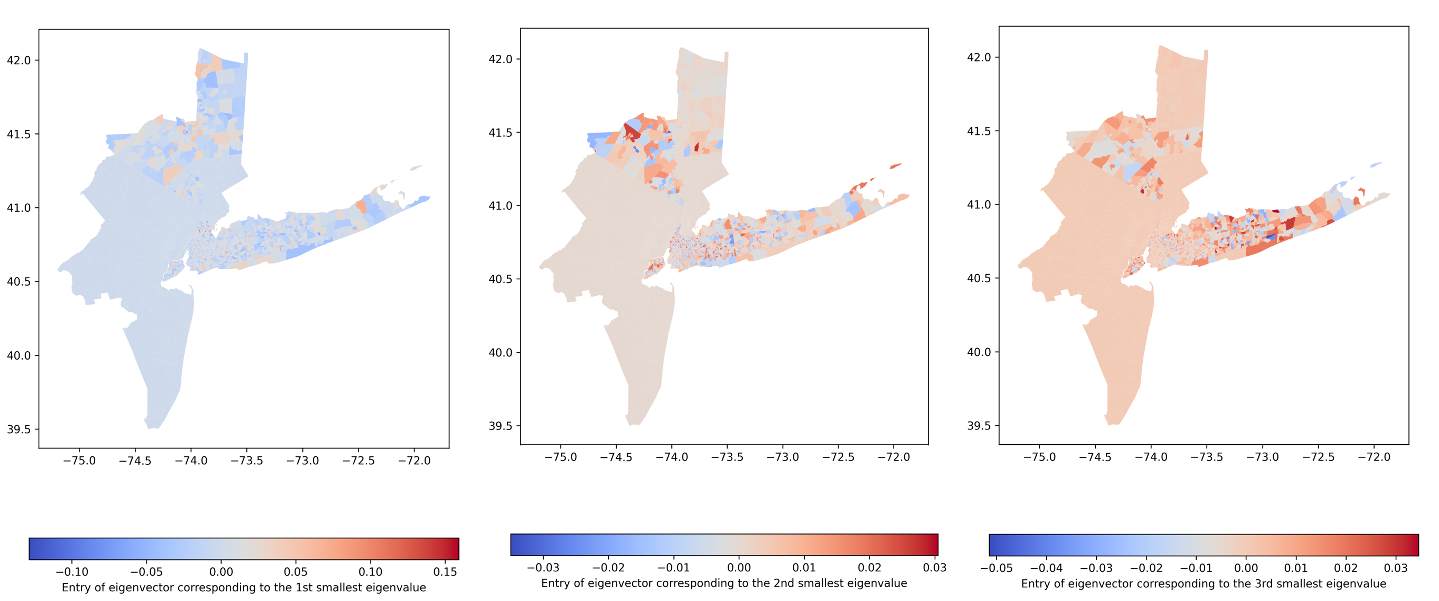
\includegraphics[width = 0.99\linewidth]{Figs/diffusionmap.png}
    \caption{扩散映射方法下,人口统计相关矩阵的前三小的正特征值对应的特征向量的空间分布。分别对应着纽约州的教育优势区域、贫困分布、和游客景点。}
    \label{fig:diffusionmap}
\end{figure}

Diffusionmap是一种流形学习方法。其出发点在于:很多多元数据的数据元只能反映客体的一部分特征,只有将多个条目的survey合起来才能得到一个比较完整的刻画。提取多个条目的survey的“权重”并不是一件简单的事,因为很多时候数据的特征是非线性变化的。这种特征往往很难用一种全局度量来衡量。流形强调的是局部性质:流形(Manifold)是局部具有欧式空间性质的空间,包括各种纬度的曲线曲面,例如球体、弯曲的平面等。流形的局部和欧式空间是同构的。流形学习假设所处理的数据点分布在嵌入于外维欧式空间的一个潜在的流形体上,或者说这些数据点可以构成这样一个潜在的流形体。流形是线性子空间的一种非线性推广。以英国的普查数据为例:英国在每个区域统计两类人口统计学指标:关键指标和快速指标。总共有1450个特征。\cite{barter2019manifold},作者用布里斯托及其周边的3490个人口统计学单元作为主要研究对象。其中的分析找到了解释统计反馈的主要变量:大学生密度和贫困程度。



\section{预期创新点}

本文通过引入较多的数学工具,对城市介观尺度下空间模式的提取、交互模式的性质、局部模式的涌现进行研究。本文的几个主要结果改进了地理大数据采集的设计,提出了定量衡量城市政策效果的方法,证明了介观尺度模式涌现的必然性。预期创新点如下:\begin{enumerate}
    \item 改进扩散映射方法,引入负相似性的概念
\end{enumerate}
\chapter{论文组织结构与时间安排}

\section{论文组织结构}

第一章为绪论,主要介绍介观尺度的地理现象,以及空间交互如何对其产生影响。本文利用高精度的交互数据和理论模型,解释了产业分化及其在空间上的固化(fixation)过程、交互模式的稳定性、以及如何从数据中提取出关键的观测维度。

第二章是利用扩散映射法提取高维地理数据的关键信息。本章首先展示扩散映射法的理论基础,近期其在城市研究中的研究进展,以及面临的问题:无法针对问题进行定制结果,以及对重复的统计量不够鲁棒。其次,我们将描述我们对上述问题的解决方案:引入多维相似性指标,进行介观降维;以及引进负相似性来描述城市空间中的相斥结构的形成机制。最后,我们将通过对英美两国的人口普查数据的改进扩散映射结果,来展示城市中一些对偶结构、特定尺度空间组织的模式发现。

第三章是城市内交互系统的稳定性分析。本章分析了城市面对外来冲击时,居民受影响程度的扩散状况。首先我们根据城市元人口交互矩阵和冲击向量构建了交互的扩散矩阵,并由此定义城市交互稳定性。进而,我们找到了一些交互系统的一些守恒量和稳定性的确定条件。最后,我们根据美国15个主要城市2020年的人类移动性数据量化了新冠病毒肺炎在各个城市内部传播的稳定性时序变化。我们的结论证明随着发病率的提高,控制城市介观结构之间的交互已经于事无补。只有严格的居家令才能使得疫情得到控制。

第四章是从众心理驱动下的介观模式形成。我们通过考察三元关系传播意愿-二元关系传播疾病的模型,反映了心理因素对二元关系的影响。我们通过主方程的方法构建了一个患病比例和戴口罩比例共同演化的非线性系统。并通过对其$(0,0)$, $(1,0)$, $(0,1)$, $(1,1)$附近稳定性的讨论,得到了一个达成“社会共识”的充要条件。最后,我们在多种真实网络上验证了我们的结果,得到了较为一般的性质。

第五章为结论。我们以介观尺度为切入点,探究了交互模式的形成、稳定性,以及如何从数据中提取不同主题交互的模式。结合研究中的不足,为进一步研究提出展望。



\section{时间进度安排}

2021 年 7 月,完成局部交互模式形成和交互稳定性的小论文投稿;

2021 年 11 月,整理相关领域研究工作及最新进展,归纳总结现存研究问题,根据开题报告答辩情况完善研究框架;

2021 年 12 月至 2022 年 6 月,根据研究计划进行具体的工作,整理实验结果,完成博士论文初稿;

2022 年 10 月,结合导师意见完善博士论文;

2023 年 4 月,完成博士论文,开展博士论文答辩工作;

2023 年 5 月至 2023 年 6 月,参照评审意见对博士论文进行修改,并完成学位论文提交。





\addcontentsline{toc}{chapter}{参考文献} %向目录中添加条目,以章的名义
\bibliographystyle{apalike}
\bibliography{ref.bib}

\addcontentsline{toc}{chapter}{附录}
\chapter*{附录}

\section*{扩散映射的数学基础}

扩散映射的方法来源于数学中网络上的扩散过程。我们考虑一个复杂网络$G(V,E)$,其上有足够多的人在进行随机游走. 每个节点$i$上分配一个随机过程$x_i(t)$, 它可以代表$t$时刻恰好处于节点$i$上的人数。每一个人都以同样的概率$1/k_i$访问所处节点$i$的邻居,其中$k_i$是节点$i$的度。于是节点上人数随时间的变化可以写成一个微分方程\begin{equation}
    \dot{x}_i = -k_i x_i + \sum_{j\to i} x_j \\
    = -k_i x_i +\sum_{j \ne i} A_{ij} x_j,
\end{equation} 其中$A$是复杂网络的邻接矩阵。我们试图找到一个矩阵$L$, 使得网络上的动态可以用方程\begin{equation}
    \dot{X} = - L X
    \label{eq:dynamic_laplacian}
\end{equation}来表示,其中$X(t) = (x_1(t), x_2(t), \dots, x_n(t))$。于是容易得到$L_{ij} = \delta_{ij}k_i - A_{ij}$. 我们称这个矩阵$L$为Laplace矩阵,并记它的特征值为$\lambda_n$, 对应的特征向量为$v_n$, $n = 1,2,3,\dots$. 根据基本的线性代数知识,我们有\begin{equation}
    Lv_n = \lambda_n v_n.
    \label{eq:eigen}
\end{equation} 这一组特征向量可以作为一组基,唯一表示所有的$n$维向量。特别的,可以表示$X(t) = (x_1(t), x_2(t), \dots, x_n(t))$为\begin{equation}
    x_n = \sum_n c_n v_n, 
    \label{eq:representation}
\end{equation}其中$c_n$为系数。将 (\ref{eq:eigen}), (\ref{eq:representation})代入 (\ref{eq:dynamic_laplacian}), 可得\begin{align}
        \partial_t \sum c_n(t)v_n = -L\sum c_n(t) v_n\\
        = -\sum c_n(t)\lambda_n v_n.
\end{align}根据唯一表示定理,每个特征向量$v_n$在等式两边的系数也是相等的,即\begin{equation}
    \dot{c}_n = -cn\lambda_n,\quad \forall n.
\end{equation}可以容易地解出每一个$c_n(t) = c_n(t) e^{-\lambda_n t}$. 进而系统可以写成:\begin{equation}
    x(t) = \sum_n c_n(t) v_n = \sum_n c_n(0)e^{-\lambda_n t} v_n. 
    \label{eq:repre}
\end{equation}真实的扩散过程转移概率都是非负的,所以特征值$\lambda_{n}$都非负。而行和又都是$0$, 所以Laplace矩阵$L$都存在一个$0$特征值为$0$, 其对应的特征向量为$(1,1,\dots, 1)^{T}$. 该特征向量只保证了矩阵的归一性,而不包含其他信息。公式 (\ref{eq:repre})告诉我们,对于一个Laplace动力系统来说,最小的特征值和其对应的特征向量是最重要的。因为系统沿着该特征向量方向收敛的速度是最慢的,可以在更长的时间尺度上保留这个方向上的性质。
\end{document}